\chapter{Arbeitsmarkt der Zukunft}\label{ch:K07_Arbeitsmarkt}

\begin{myremark}
KI verändert den Arbeitsmarkt fundamental. Dieses Kapitel beleuchtet, welche Berufe
besonders betroffen sind, welche neuen Berufsfelder entstehen und wie Sie sich in
einer KI-geprägten Berufswelt positionieren können.
\end{myremark}

\section{Welche Berufe verändern sich durch KI?}

\begin{myexample}
Historisch haben technologische Revolutionen immer Berufe verändert:
\begin{itemize}
    \item Die \textbf{Industrialisierung} ersetzte viele manuelle Berufe durch
          Maschinen, schuf aber auch neue Berufe (Maschinentechniker, Ingenieure).
    \item Die \textbf{Digitalisierung} veränderte Büroarbeit fundamental
          (Schreibmaschinen-Schreiberinnen verschwanden, IT-Fachleute entstanden).
    \item \textbf{KI} könnte ähnliche Auswirkungen auf Wissensarbeit haben.
\end{itemize}
\end{myexample}

\begin{mydefinition}
Zwei wichtige Konzepte zur Einschätzung des KI-Einflusses auf Berufe:
\begin{itemize}
    \item \textbf{Automatisierbarkeit}: Wie leicht kann eine Aufgabe vollständig
          von KI übernommen werden?
    \item \textbf{Augmentation}: Wie stark kann KI eine menschliche Arbeit
          \emph{ergänzen} und verbessern, ohne sie zu ersetzen?
\end{itemize}
\end{mydefinition}

\begin{myoverview}[Berufe und KI-Exposition]
\begin{center}
\begin{tabular}{p{4cm}p{4cm}p{5cm}}
    \toprule
    \textbf{Hoch exponiert}      & \textbf{Mittel exponiert}     & \textbf{Wenig exponiert}      \\
    (Automatisierungsgefahr)     & (Veränderung + Augmentation)  & (Schwer automatisierbar)      \\
    \midrule
    Dateneingabe                 & Buchhalter/-in                & Pflegefachperson              \\
    Einfache Textproduktion      & Journalistin / Journalist     & Sozialarbeiterin / -arbeiter  \\
    Callcenter-Agent/-in         & Grafikdesigner/-in            & Handwerksberufe               \\
    Übersetzung (Standard)       & Lehrkraft                     & Sportcoach/-trainerin         \\
    Routineanalysen              & Softwareentwickler/-in        & Künstlerin / Künstler         \\
    \bottomrule
\end{tabular}
\end{center}
\end{myoverview}

\begin{myexercise}[Berufsanalyse]
Wählen Sie einen Beruf, der Sie interessiert. Recherchieren Sie (optional: nutzen
Sie ein KI-Tool), welche Aufgaben in diesem Beruf:
\begin{itemize}
    \item heute schon durch KI automatisiert werden können,
    \item durch KI \emph{unterstützt} (augmentiert) werden könnten,
    \item dauerhaft menschliche Kompetenz erfordern werden.
\end{itemize}

Halten Sie Ihre Ergebnisse in einer Tabelle fest und präsentieren Sie diese
in 3 Minuten der Klasse.
\end{myexercise}

\section{Neue Berufsfelder durch KI}

\begin{myexample}
Berufe, die durch KI neu entstanden sind oder stark gewachsen sind:
\begin{itemize}
    \item \textbf{Prompt Engineer}: Spezialisiert auf das Formulieren effektiver
          Prompts für grosse Sprachmodelle.
    \item \textbf{AI Safety Researcher}: Forscht daran, KI-Systeme sicher und
          verlässlich zu machen.
    \item \textbf{KI-Ethiker/-in}: Bewertet gesellschaftliche Auswirkungen von
          KI-Systemen und entwickelt ethische Leitlinien.
    \item \textbf{Data Annotator / AI Trainer}: Bewertet und beschriftet Daten,
          die zum Training von KI-Modellen verwendet werden.
    \item \textbf{MLOps Engineer}: Zuständig für den Betrieb und die
          Skalierung von ML-Modellen in der Produktion.
    \item \textbf{Human-AI Interaction Designer}: Gestaltet die
          Schnittstelle zwischen Mensch und KI-System.
\end{itemize}
\end{myexample}

\section{Auftrag: Präsentation zum Arbeitsmarkt der Zukunft}

\begin{myexercise}[PPT-Auftrag: Arbeitsmarkt]
\textbf{Gruppenauftrag}: Sie erstellen in Zweiergruppen eine Präsentation
(8--10 Folien, ca. 10 Minuten Präsentation) zum Thema

\begin{center}
    \enquote{Wie verändert KI den Arbeitsmarkt in meinem Interessensbereich?}
\end{center}

\textbf{Grundlage}: Lesen Sie zunächst die bereitgestellten NZZ-Artikel
(s.\,u.) und nutzen Sie diese als Hauptquellen. Ergänzen Sie Ihre Recherche
mit weiteren seriösen Quellen.

\medskip
\textbf{Pflichtstruktur der Präsentation}:
\begin{enumerate}
    \item \textbf{Titelfolie} mit Thema, Namen, Datum
    \item \textbf{Ausgangslage}: Wie sieht der Beruf / das Berufsfeld heute aus?
    \item \textbf{KI-Disruption}: Welche konkreten KI-Anwendungen verändern
          dieses Berufsfeld bereits heute?
    \item \textbf{Chancen}: Welche neuen Möglichkeiten entstehen durch KI?
    \item \textbf{Risiken}: Welche Risiken und Herausforderungen entstehen?
    \item \textbf{Fallbeispiel}: Ein konkretes Unternehmen oder eine Person,
          die KI in diesem Berufsfeld nutzt.
    \item \textbf{Ausblick 2030}: Wie könnte der Beruf in 5 Jahren aussehen?
    \item \textbf{Persönliche Relevanz}: Was bedeutet das für Sie persönlich?
          Welche Kompetenzen wollen Sie aufbauen?
    \item \textbf{Quellen} (mind. 3, davon mindestens 1 NZZ-Artikel)
\end{enumerate}

\textbf{Bewertungskriterien}:
\begin{itemize}
    \item Inhaltliche Tiefe und Korrektheit
    \item Eigenständige Reflexion (nicht nur zusammengefasst)
    \item Quellenqualität und -vielfalt
    \item Präsentationsqualität (Struktur, Visualisierung, Redeweise)
\end{itemize}
\end{myexercise}

\subsection*{NZZ-Artikel: Arbeitsmarkt und KI}

\begin{figure}[H]
      \centering
      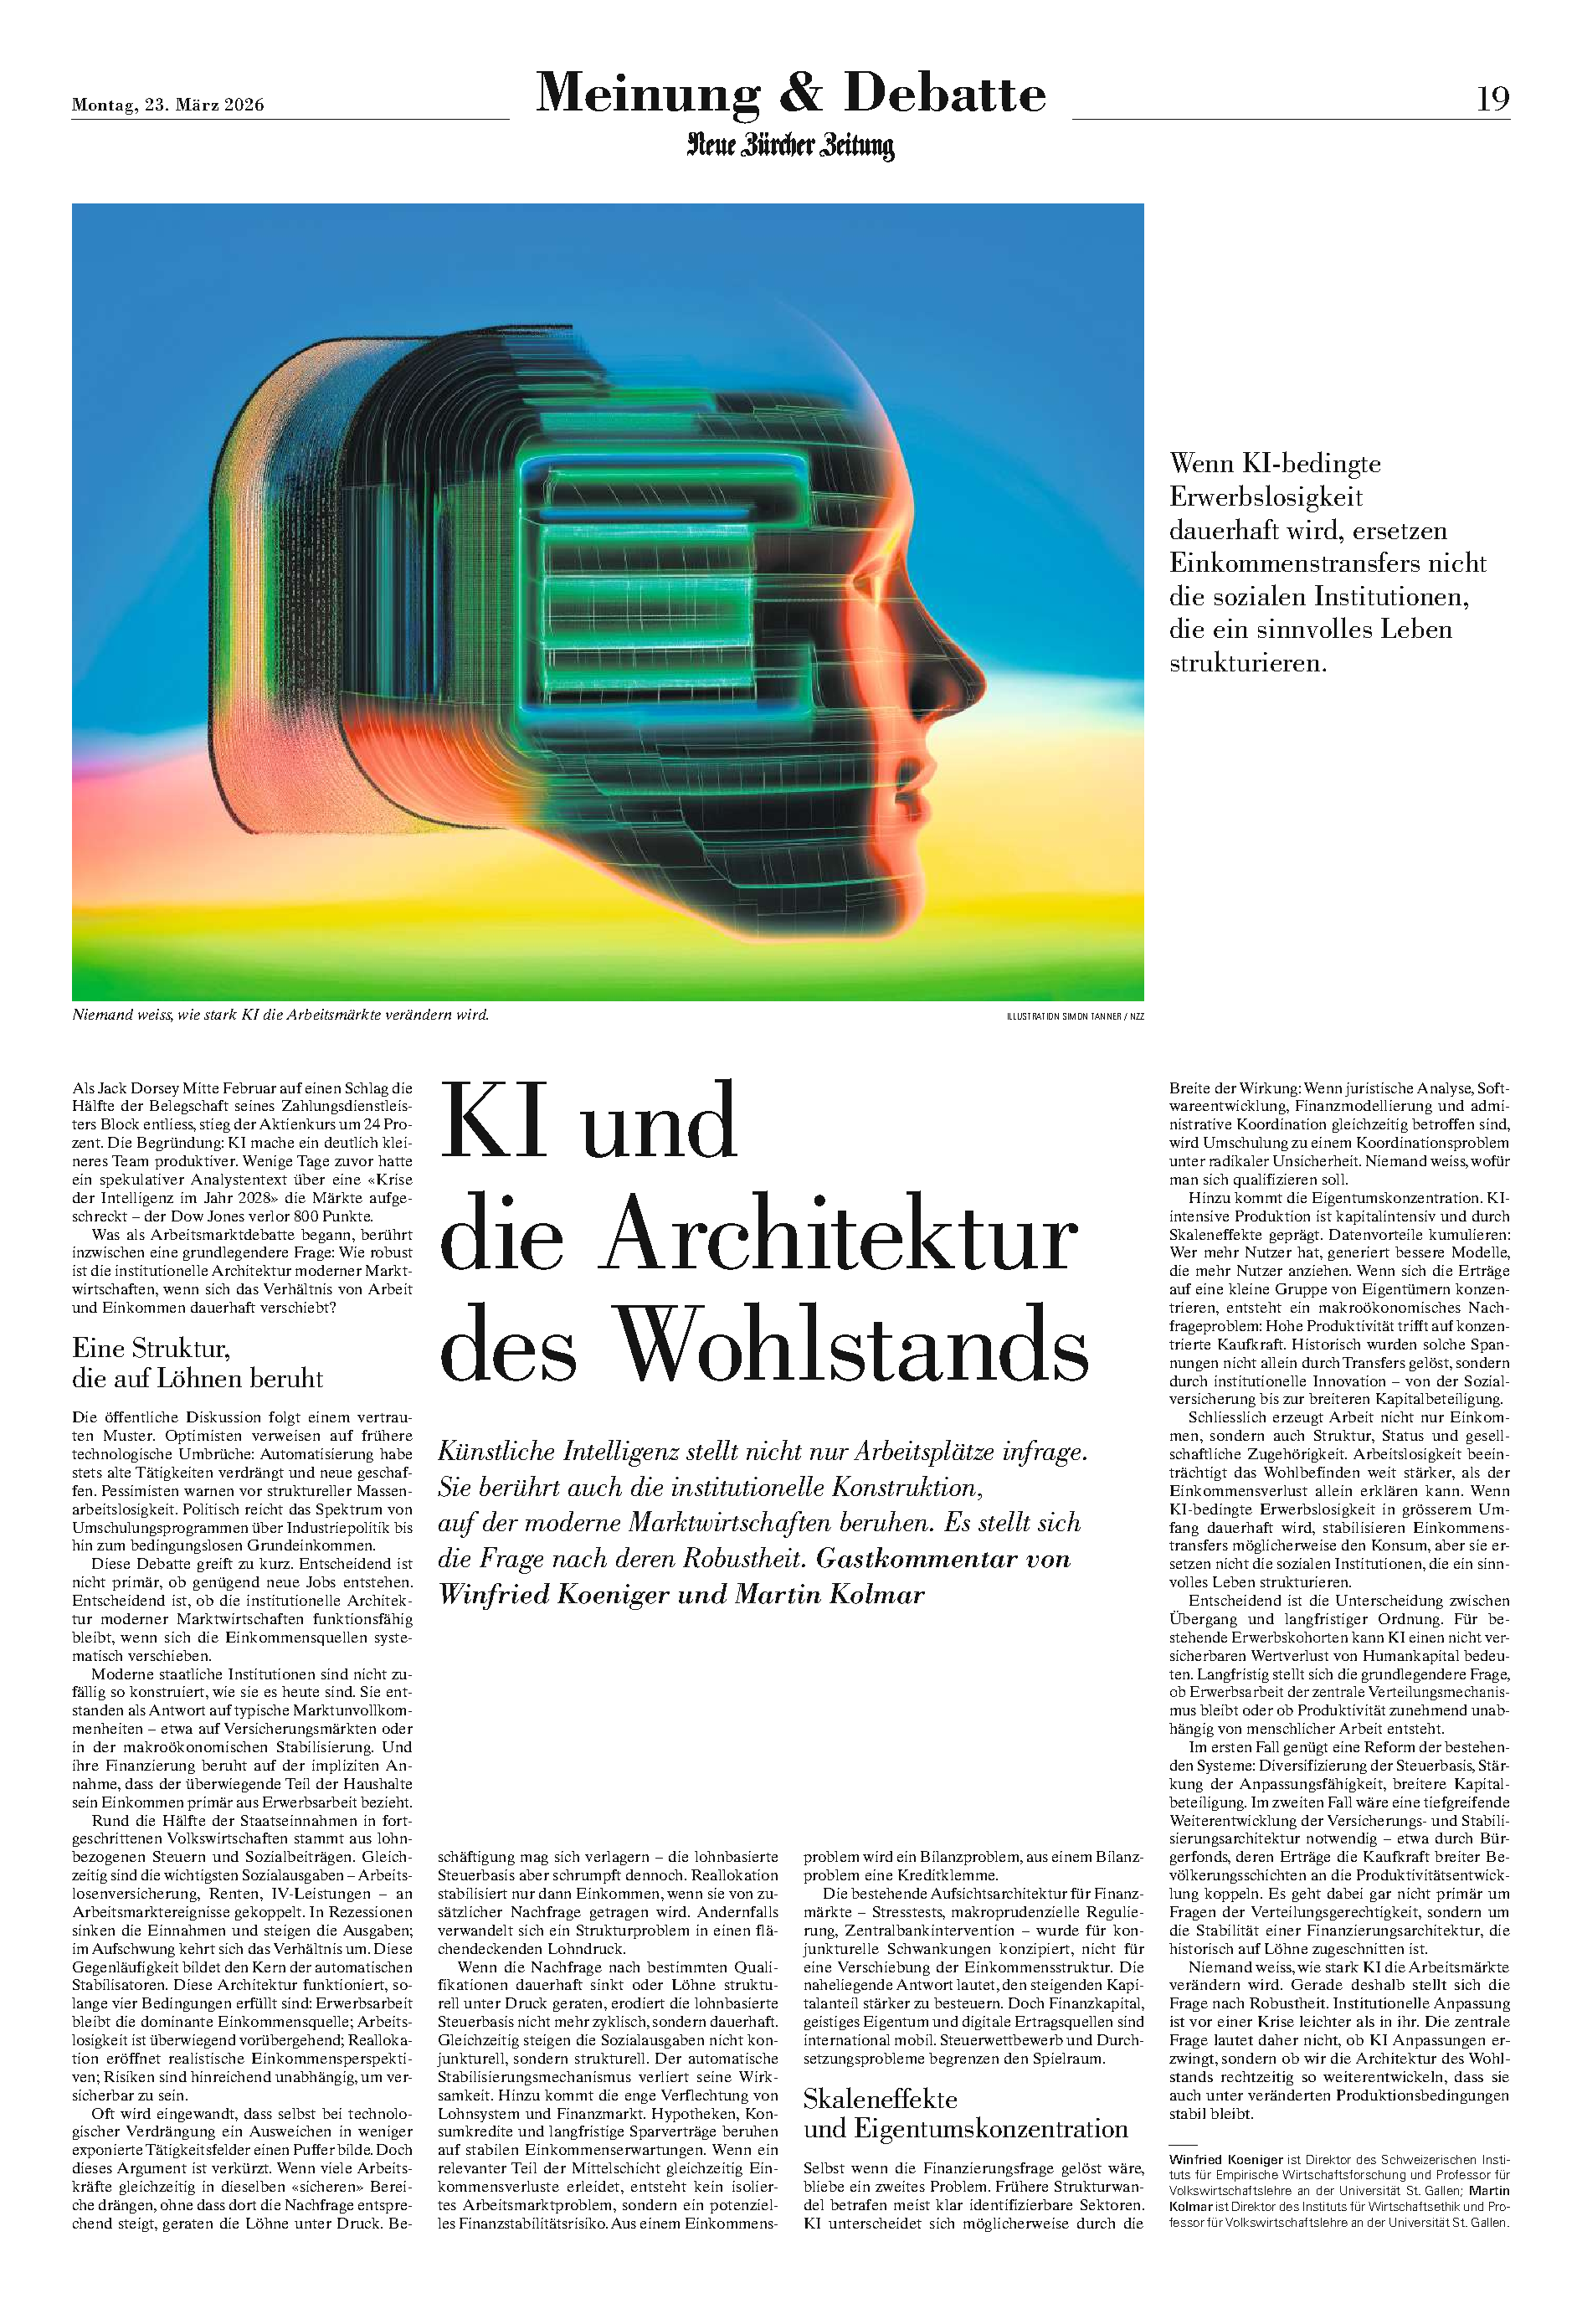
\includegraphics[width=\textwidth]{Grundlagen_Info/14_KI_und_Prompting/Articles/2026-03-26 NZZ KI Einfluss auf Wirtschaft und Massnahmen.pdf}
\end{figure}


\begin{figure}[H]
      \centering
      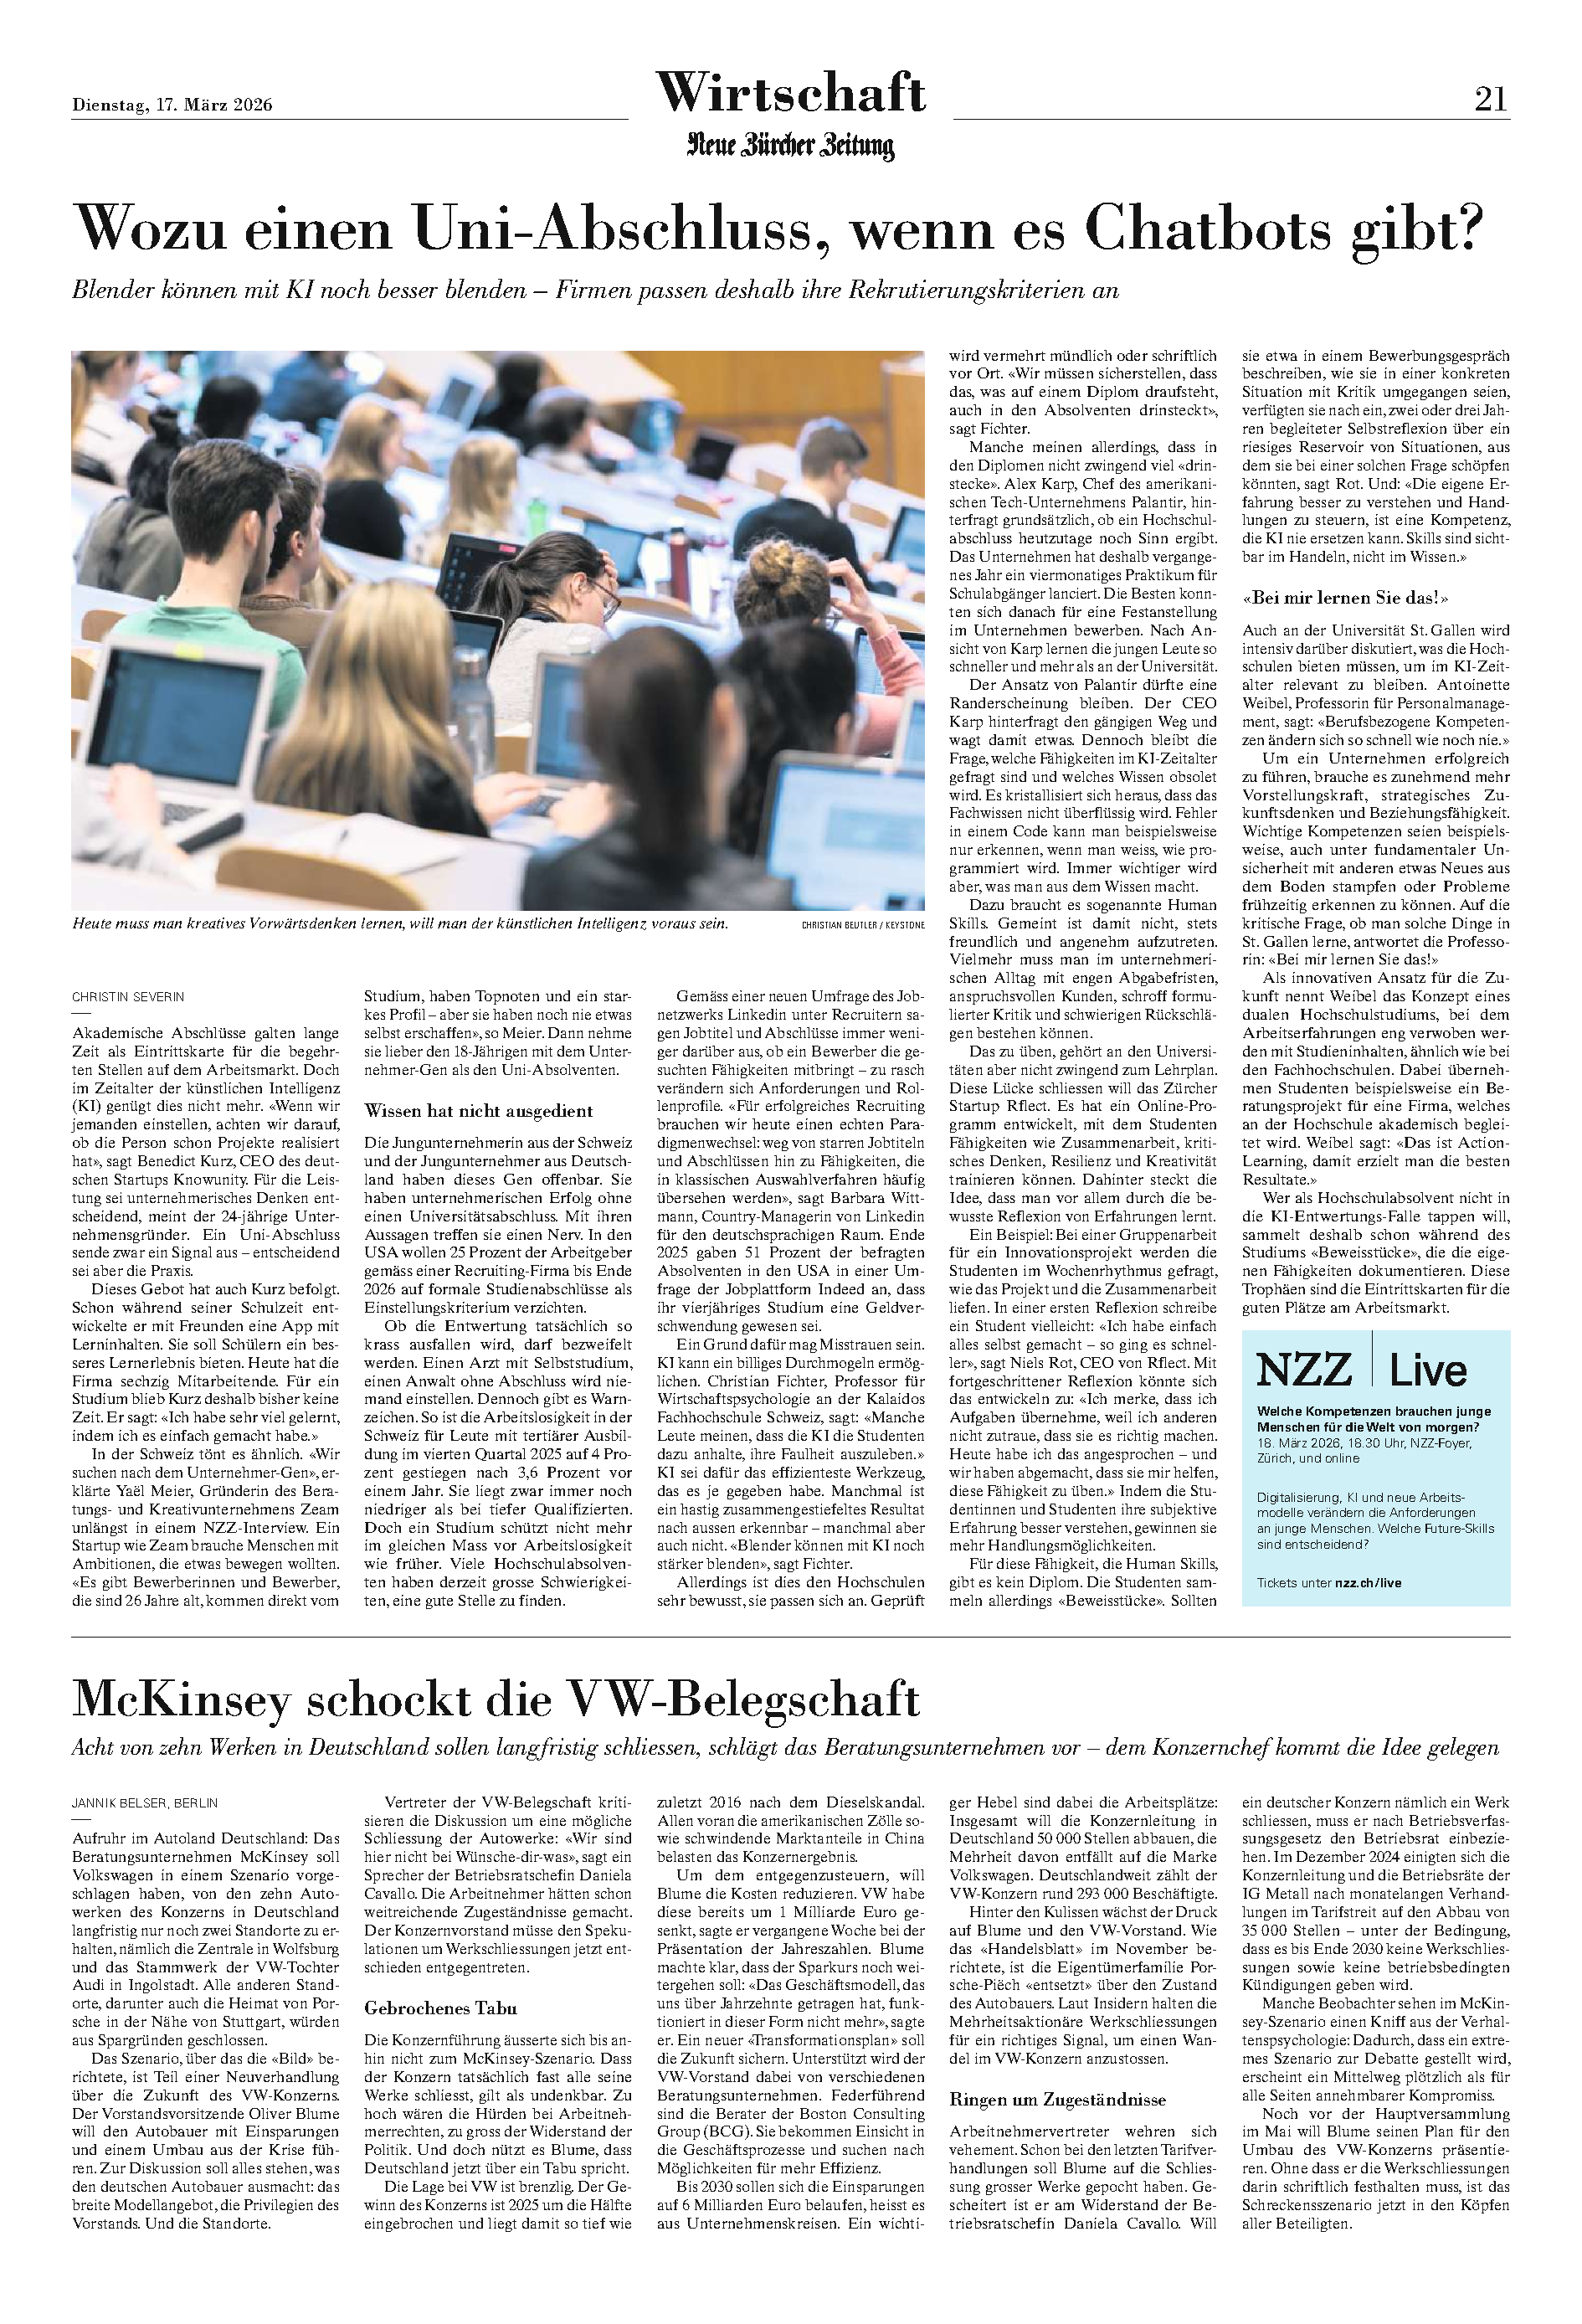
\includegraphics[width=\textwidth]{Grundlagen_Info/14_KI_und_Prompting/Articles/2026-03-17 NZZ Universitäten KI.pdf}
\end{figure}


\section{Welche Kompetenzen bleiben zukunftssicher?}

\begin{mysummary}
Kompetenzen, die durch KI schwer zu ersetzen sind:
\begin{itemize}
    \item \textbf{Kritisches Denken}: Bewertung und Hinterfragen von
          Informationen --- auch KI-generierter.
    \item \textbf{Kreativität und Originalität}: Echte Neuideen,
          künstlerischer Ausdruck.
    \item \textbf{Emotionale Intelligenz}: Empathie, Teamarbeit,
          Konfliktlösung.
    \item \textbf{Komplexe Problemlösung}: Aufgaben, die mehrere Domänen
          und unstrukturiertes Wissen erfordern.
    \item \textbf{Prompt Literacy}: Die Fähigkeit, KI effektiv und kritisch
          einzusetzen.
    \item \textbf{Lebenslanges Lernen}: Bereitschaft, sich laufend neu
          anzupassen.
\end{itemize}
\end{mysummary}

\begin{myexercise}[Reflexion: Meine Zukunft]
Schreiben Sie einen kurzen persönlichen Reflexionstext (ca. 200 Wörter) zu
folgenden Fragen:

\begin{itemize}
    \item Welchen Beruf strebe ich an --- oder welche Berufsfelder interessieren
          mich?
    \item Wie schätze ich das KI-Automatisierungsrisiko für diesen Bereich ein?
    \item Welche Fähigkeiten möchte ich in den nächsten Jahren entwickeln,
          um zukunftssicher zu sein?
    \item Sehe ich KI eher als Chance oder als Bedrohung für meine berufliche
          Zukunft? Warum?
\end{itemize}
\end{myexercise}

\begin{mychallenge}[KI-Karriereberatung]
\begin{myattention}
\textbf{Optional --- Eigenverantwortung}: Nutzung von ChatGPT / Claude auf eigene
Verantwortung. Keine persönlichen Daten eingeben.
\end{myattention}

Nutzen Sie ein LLM als Karriereberaterin: Geben Sie Ihre Interessen und
bisherigen Stärken ein (ohne echten Namen) und bitten Sie das Modell,
drei Berufsfelder vorzuschlagen, in denen Ihre Kompetenzen in einer
KI-geprägten Welt besonders gefragt sein werden.

Bewerten Sie kritisch: Sind die Vorschläge des Modells realistisch?
Was fehlt der KI, um wirklich gute Karriereberatung zu leisten?
\end{mychallenge}
